\chapter{Docker Network}
\section{Pengertian}
Dikutip dari situs Docker Docs, Docker network merupakan sistem jaringan docker untuk menghubungkan antar container docker atau menghubungkannya ke beban kerja non-docker.
Kontainer dan layanan docker bahkan tidak perlu menyadari bahwa mereka di deploy di docker, atau apakah container/layanan docker lain merupakan beban kerja docker atau tidak.
Baik host docker pengguna menjalankan linux, windows atau campuran keduanya, pengguna dapat menggunakan docker untuk mengelolanya dengan cara diagnostik platform.

\section{Docker Network Drivers}
Subsistem docker network dapat dihubungkan menggunakan driver. Beberapa driver ada secara default dan menyediakan fungsionalitas jaringan inti diantaranya :
\subsection{Bridge (default)}
merupakan konfigurasi default server docker network jika pengguna tidak mendefinisikan driver saat membuat docker network. Bridge biasanya digunakan saat aplikasi 
yang berjalan dalam kontainer secara mandiri perlu berkomunikasi. Pengguna dapat menggunakan driver ini untuk komunikasi antara kontainer dalam docker host yang sama.
\subsection{Host}
merupakan konfigurasi untuk kontainer mandiri, menghapus isolasi jaringan antara kontainer dan docker host, dan menggunakan jaringan host secara langsung. Pengguna dapat menggunakan driver ini
ketika tumpukan jaringan tidak boleh diisolasi dari docker host tapi mengiginkan aspek lain dari kontainer untuk diisolasi.
\subsection{Overlay}
merupakan konfigurasi untuk menghubungkan beberapa docker daemon bersama sama dan memungkinkan layanan swarm untuk berkomunikasi satu sama lain. Strategi ini menghilangkan kebutuhan untuk melakukan perutean tingkat OS diantara kontainer.
Pengguna dapat menggunakan driver ini untuk komunikasi antara kontainer dalam host docker yang berbeda atau saat beberapa aplikai bekerja sama menggunakan layanan swarm.
\subsection{IPvlan}
merupakan konfigurasi yang memberi pengguna kendali penuh atas pengalamatan IPv4 dan IPv6. Driver VLAN dibangun diatas itu dan memberi pengguna kendali penuh pada lapisan 2 VLAN tagging bahkan IPvlan L3 untuk 
pengguna yang tertarik pada integrasi jaringan underlay.
\subsection{Macvlan}
merupakan konfigurasi yang memperbolehkan pengguna untuk memasukan MAC Address ke kontainer, dan membuatnya tampak sebagai perangkat fisik di jaringan. Daemon docker merutekan lalu lintas ke kontainer dengan MAC Address.
Pengguna dapat menggunakan driver ini agar kontainer terlihat seperti host fisik di jaringan, masing masing dengan MAC Address yang unik.
\subsection{None}
merupakan konfigurasi untuk menonaktifkan semua jaringan , biasanya digunakan bersama dengan driver jaringan khusus.
\subsection{Network Plugins}
merupakan konfigurasi untuk menginstal dan menggunakan plugin jaringan pihak ketiga dengan Docker. Plugin ini tersedia dari docker hub atau vendor pihak ketiga. 

\begin{figure}
    Pengguna dapat melihat port jaringan khusus untuk docker dalam linux 
    COMMAND: \textcolor{Blue}{ifconfig}
    \begin{center}
        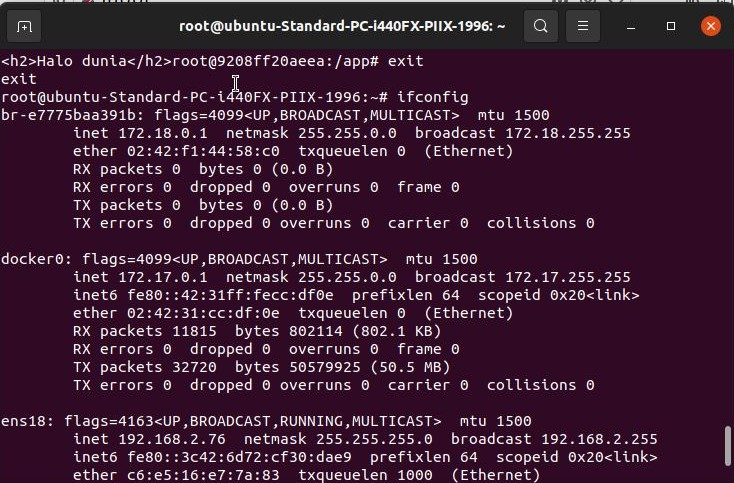
\includegraphics[width=\linewidth]{image/49.jpg}
        \caption{Lihat port jaringan}
        \label{fig:my_figure}
    \end{center}

\end{figure}
